\chapter{Structural Typing}
\label{chapter:StructuralTyping}
\lhead{ \leftmark }

A type system that requires equivalent types to have the same declared name, regardless of whether they define identical fields and methods, is referred to as a \emph{nominal} (or \emph{nominative}) type system.  A type system that ignores the declared name of types and only requires equivalent types to share common field or method declarations is referred to as a \emph{structural} type system.  More formally, for types $T_0$ and $T_1$, in a nominal type system $T_0 \equiv T_1 \iff {T_0}_{name} = {T_1}_{name}$. In a structural type system $T_0 \equiv T_1 \iff \forall \; F \in {T_0}_{SLOTS} \; \exists \; F' \in {T_1}_{SLOTS}, F_{TYPE} \equiv {F'}_{TYPE} $ where slots can be a field or method defined within the given type.

\section{Nominal Typing}

As described in chapter \ref{chapter:JVM}, the JVM uses nominal types throughout.  Type names are declared in Java source, embedded into bytecode instructions, and enforced at runtime by the JVM.  As shown in Listing \ref{types-nominal}, even though classes \texttt{A} and \texttt{B} are structurally identical, they are not considered equivalent within Java or by the JVM at runtime, and therefore cannot be used interchangeably.

\begin{lstlisting}[language=Java,caption=Nominal types,label=types-nominal]
  class A {
    void test() { ... }
  }
  class B {
    void test() { ... }
  }
  void m1(A a) {
    a.test();
    m2(a);      // illegal
  }
  void m2(B b) {
    b.test();
    m1(b);      // illegal
  }
\end{lstlisting}


\subsection{Case Study: java.io.Closeable}

Prior to the release of J2SE 1.5 in 2004, the Java standard library developers noticed they had several classes in the \texttt{java.io} package that all had \texttt{close()} methods.  They wanted to be able to write generalized code that could operate on all of these classes, but the classes all had different hierarchies -- they extended different base classes -- so they could not be addressed as one common type.  To solve this problem, the \texttt{java.io.Closeable} interface was introduced.  This interface defines only a \texttt{close()} method that throws an \texttt{IOException}, and is meant to enables objects that represented resources such as files and network connections to be closed without the caller knowing anything about the class implementation other than the fact that it implements \texttt{close()}.

However, this presented a problem when dealing with the large collections of code already written.  Existing classes that had \texttt{close()} methods but did not explicitly implement the \texttt{Closeable} interface -- because it didn't exist when the code was written -- could not be passed as an argument to code expecting an instance of \texttt{Closeable}.  Due to Java's nominal type system, existing code would have to be modified to add the \texttt{implements Closeable} declaration to every relevant class definition and then be recompiled and released as a new version.

One solution to the \texttt{Closeable} problem would be to create a way for classes that do not explicitly implement the \texttt{Closeable} interface to still be treated as equivalent to the \texttt{Closeable} interface as long as they implement that single \texttt{close()} method.  That concept is a form of structural typing.

\section{Structural Typing}

Listing \ref{types-structural} demonstrates both the benefits and potential pitfalls of structural typing.  Similar to Listing \ref{types-nominal}, two structurally equivalent types are defined.  The difference is that, since \texttt{Cowboy} and \texttt{Rectangle} are structurally identical and they are defined within a structural type system, they can be used interchangeably on lines 9 and 13.

\begin{lstlisting}[language=Java,caption=Structural types,label=types-structural]
  class Cowboy {
    void draw() { ... }
  }
  class Rectangle {
    void draw() { ... }
  }
  void drawGun(Cowboy cowboy) {
    cowboy.draw();
    paint(cowboy);      // legal
  }
  void paint(Rectangle rect) {
    rect.draw();
    drawGun(rect);      // legal
  }
\end{lstlisting}

This approach solves the \texttt{java.io.Closeable} problem.  Code could be written within this system that operated on both the \texttt{Cowboy} and \texttt{Rectangle} types uniformly, even though they have no explicitly declared relation to one another.  New interfaces can be written that existing classes implicitly implement without modification.  However, this interchangeable usage should immediately be cause for concern.  The \texttt{draw()} method in Listing \ref{types-structural}, while lexically identical in each class, has a different meaning within the domain of each class.  In the context of a \texttt{Cowboy}, to \texttt{draw()} means to draw a gun.  In the context of a \texttt{Rectangle}, \texttt{draw()} means to render itself.  This is an example of the ambiguity of the English language leaking into what should be a more formal definition within a programming language.  This \emph{accidental equivalence}, an edge case within structural type systems, can be mitigated through a hybrid use of structural typing with \emph{structural interfaces}.

\subsection{Structural Interfaces}

There is a design compromise between structural typing and nominal typing that solves the \texttt{java.io.Closeable} problem while minimizing accidental equivalence.  Described with Java-like syntax in Listing \ref{types-structural-interfaces}, the hybrid approach uses nominal typing to determine equivalence of two classes and structural typing to determine whether a type conforms to an interface.

\begin{lstlisting}[language=Java,caption=Structural interface,label=types-structural-interfaces]
  class Cowboy {
    void draw() { ... }
    int getHeight() { ... }
  }
  class Rectangle {
    void draw() { ... }
    int getHeight() { ... }
  }
  interface Height {
    int getHeight();
  }
\end{lstlisting}

In Listing \ref{types-structural-interfaces}, \texttt{Cowboy} and \texttt{Rectangle} both conform to the \texttt{Height} interface by implementing the \texttt{getHeight()} method and can be provided to any receiver that is expecting an instance of \texttt{Height}.  However, even though \texttt{Cowboy} and \texttt{Rectangle} have identical structures they are not equivalent to each other and cannot be used interchangeably, thereby limiting accidental equivalence errors.

\section{Implementation}

The implementation challenges of structural interfaces stem from the fact that each concrete type (a type that corresponds to a specific memory layout) has the potential to implicitly implement a large number of interfaces.  An interface like \texttt{java.io.Closeable} in a structural type system could be implemented by hundreds of concrete types, so when a function accepts an instance of \texttt{java.io.Closeable} as a parameter and calls its \texttt{close()} method the compiler has no idea which of the hundreds of implementing types will be passed to the function at runtime.  If the fields and methods of a concrete type are generalized as \emph{slots} (an offset within the memory layout of the concrete type), the problem can be described as whether the compiler can calculate the offset of a slot based only on information available at the call site at compile time, or if the offset of the slot cannot be determined until runtime.

\subsection{Compile-Time Slot Lookup}

Each name of a class in Java corresponds to one and only one memory layout of the fields and methods of that class.  Listing \ref{code-layout-nominal} defines several Java classes, and Figure \ref{fig:memory-layout-nominal} shows an approximation of the corresponding memory layout.

\begin{lstlisting}[language=Java,caption=Nominal type inheritance,label=code-layout-nominal]
  class Base {
    void sayHello() { ... }
  }
  class Class1 extends Base {
    void m1() { ... }
    void sayHello() { ... }
  }
  class Class2 extends Base {
    void m2() { ... }
    void sayHello() { ... }
    void m3() { ... }
  }
  class Class3 extends Class2 {
    void m2() { ... }
    void sayHello() { ... }
    void m4() { ... }
  }
\end{lstlisting}

\begin{figure}[htbp]
  \centering
    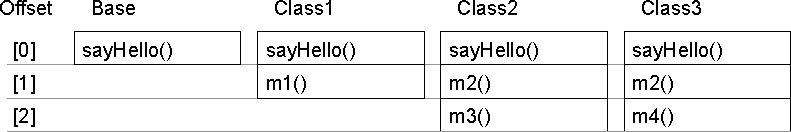
\includegraphics[width=\textwidth]{./Figures/memory-layout-nominal.pdf}
  \caption[Single Inheritance Memory Layout]{An abstract representation of class memory layout.}
	\label{fig:memory-layout-nominal}
\end{figure}

Given a pointer to an instance of \texttt{Base}, the compiler knows at compile time that \texttt{sayHello()} will always be located at offset \texttt{[0]}.  The same relationship exists between \texttt{Class2} and its subclass, \texttt{Class3}.  Given a pointer to any class that extends \texttt{Class2}, \texttt{m2()} will always be at offset \texttt{[1]}.  Each subclass aligns its lower offsets with its base class structure, then uses its higher offsets for its own structure.  This predictability enables a compiler to calculate the offset of any field or method of a class and generate a simple indirect load or jump instruction to access it.

\subsection{Runtime Slot Lookup}

Listing \ref{code-layout-structural} shows pseudocode of two interfaces and two classes.  \texttt{Class1} and \texttt{Class2} both implement the \texttt{Stream} interface by implementing \texttt{close()}.  \texttt{Class2} also implements the \texttt{Gettable} interface by implementing \texttt{get()}.

\begin{lstlisting}[language=Java,caption=Pseudocode: Java with structural types,label=code-layout-structural]
  interface Gettable {
    void get();
  }
  interface Stream {
    void close();
  }
  class Class1 {
    void close() { ... }
  }
  class Class2 {
    void close() { ... }
    void get() { ... }
  }
  void call( Stream stream ) {
    stream.close();
  }
\end{lstlisting}

\begin{figure}[htbp]
  \centering
    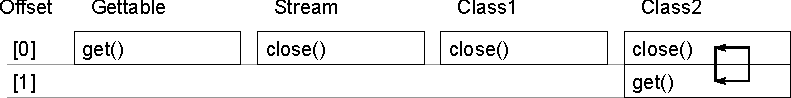
\includegraphics[width=\textwidth]{./Figures/memory-layout-structural.pdf}
  \caption[Structural Inheritance Layout]{An abstract representation of class memory layout.}
	\label{fig:memory-layout-structural}
\end{figure}

When calling into concrete types, the offset of a given method was known at compile time.  With structural typing this is no longer the case, as evident by the memory layout of \texttt{Class2} in Figure \ref{fig:memory-layout-structural}.  Since \texttt{Class2} implements both the \texttt{Gettable} and \texttt{Stream} interfaces it must allocate a slot in its memory layout for both the \texttt{get()} and \texttt{close()} methods.  However, both of those methods are defined at offset \texttt{[0]} in their respective interfaces.  If a compiler places the \texttt{close()} method at offset \texttt{[0]} of \texttt{Class2}, any call sites receiving an instance of \texttt{Class2} as a \texttt{Gettable} cannot predict at compile time the offset at which the \texttt{get()} method will be located.  The inverse is also true if the \texttt{get()} method was placed at offset \texttt{[0]}.  This problem is aggravated when more than two interfaces are considered across multiple concrete types.

The offset that must be resolved on the receiver from the call site on line 15 cannot be determined through static analysis.  The call site could be provided either \texttt{Class1} or \texttt{Class2} at runtime, and must be able to efficiently lookup the offset for the \texttt{close()} method on that type and invoke it.  This ad-hoc type introspection requirement has the potential to introduce significant overhead per invocation.

Prior to \texttt{invokedynamic}, the rigid nature of the invocation bytecode instructions meant the options to lookup and call methods on types at runtime were limited.  Implementing a feature like structural typing on the JVM required either reflection or a code generation technique that generated inline type checks at the call site at compile time \cite{structural-types-scala}.  Neither option was preferable, since reflection introduced significant overhead and the code generation technique cannot account for types that are unknown at compile time.

With \texttt{invokedynamic} method lookup overhead can be reduced by having the call site itself cache references to methods by receiver type as they are invoked.  This approach has the potential to completely eliminate the method lookup as long as the receiver type is in the call site cache.

\section{Inline Caching}

An \emph{inline cache} is a dispatch table embedded in a call site that builds an associative cache of receiver type metadata in order to optimize future invocations.  Inline caching was first developed for use in Smalltalk implementations in the 1980s \cite{smalltalk-pic} in order to improve dynamic invocation performance.  Listing \ref{code-interface-callsite} defines an interface call site that could benefit from inline caching.

\begin{lstlisting}[language=Java,caption=An interface call site,label=code-interface-callsite]
  interface Gettable {
    void get();
  }
  class A {
    void get() { ... }
  }
  class B {
    void get() { ... }
  }
  class C {
    void get() { ... }
  }
  void call( Gettable g ) {
    g.get();
  }
\end{lstlisting}

On the first invocation of \texttt{call(Gettable)} in Listing \ref{code-interface-callsite}, the inline cache of call site \texttt{g.get()} will be empty.  If, for example, an instance of class \texttt{A} was passed as the parameter on the first invocation, a full lookup would have to be performed to examine the methods implemented in class \texttt{A} and find \texttt{get(Greetable)}.  Once it is resolved, however, the offset of \texttt{get()} within class \texttt{A} will be added to the inline cache as an association between the receiver type \texttt{A} and the method handle of \texttt{get()} within type \texttt{A}.

Depending on how many receivers a call site is associated with, it can be referred to as either \emph{monomorphic}, \emph{polymorphic}, or \emph{megamorphic}.
 
\subsection{Monomorphic}

According to research by Oracle's HotSpot engineering team, 90\% of call sites only target one concrete method over their entire lifetime \cite{hotspot-virtualcalls}.  These call sites, called \emph{monomorphic}, retain a reference to the previously invoked receiver type.  Upon subsequent invocation, the previous receiver type is compared to the new receiver type and, if they match, the cached receiver metadata can be used to jump directly to the target method.

The design decisions inherent to monomorphic call sites all revolve around the caching heuristics.  Primarily, what happens on a cache miss?  If a call site replaces its cached receiver type each time the new receiver doesn't match, the overhead of cache maintenance could dominate execution time if a call site is being called with two types in an alternating invocation pattern.  Conversely, choosing to not replace the cached receiver type could miss an optimization opportunity.  One approach to avoid these issues, developed as an extension to the monomorphic inline cache by Sun Microsystems for the Self project, is to simply grow the cache to accommodate new receiver types \cite{self-pic}.

\subsection{Polymorphic}

A \emph{polymorphic inline cache} is an inline cache that stores multiple receiver types.  Pseudocode for a polymorphic inline cache for the call site in Listing \ref{code-interface-callsite} is demonstrated in Algorithm \ref{algo:poly-cache}.

\begin{flushright}
\begin{algorithm}[H]
 \SetAlgoLined
 \Switch{ receiver.type }{
  \lCase{A}{ A.get()\; }
  \lCase{B}{ B.get()\; }
  \lCase{C}{ C.get()\; }
  \lOther{
    lookup(receiver)\;
  }
 }
 \label{algo:poly-cache}
 \caption{Inline cache method dispatch}
\end{algorithm}
\end{flushright}

\smallskip

For the roughly 10\% of call sites that are invoked against more than one receiver type, a polymorphic inline cache is allocated with initial space to store several receiver types.  If a new receiver type is used at the call site, it falls through to the slower \texttt{lookup()} function which performs a linear search on the receiver type for the target method, then adds it to the cache.

This behavior can be implemented with a tree of method handles as depicted in Figure \ref{fig:guard-pic}.

\begin{figure}[htbp]
	\centering
    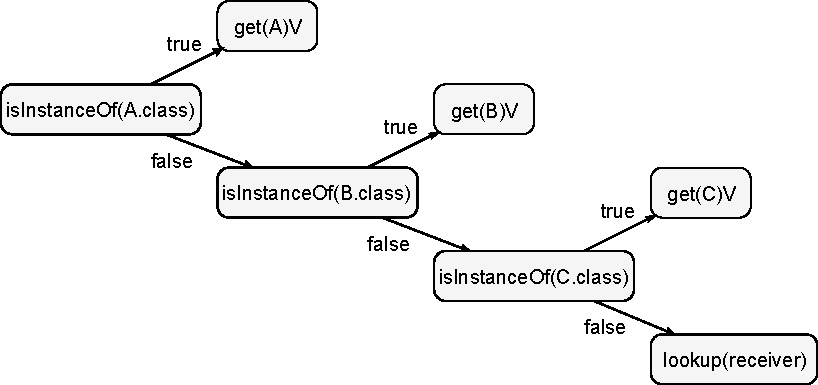
\includegraphics[width=\textwidth]{./Figures/guard-pic.pdf}
	\caption[Method Handle PIC]{A polymorphic inline cache implemented with nested method handles.}
  \label{fig:guard-pic}
\end{figure}

Constructed with the \texttt{guardWithTest()} factory method in the \texttt{MethodHandles} class, the guard is bound to the \texttt{isInstanceOf(Class)} method of the \texttt{java.lang.Class} metaclass of the receiver.  If the guard succeeds, it immediately invokes a method handle that references the concrete method.  If the guard fails, the fallback of the guard is the guard of the next receiver type check.  There are several optimization variations that influence how this tree can be constructed.  New types can be added to the root of the tree or inserted before the final \texttt{lookup(receiver)} call.  Invocation counts could be tracked, bubbling up the most invoked receiver type to the root of the tree so it is checked first in order to speed up dispatch time.  However, obviously the tree cannot grow without bound.  The inline cache must be designed to handle the 1\% of cases where an unmanageable number of types flow through one call site.

\subsection{Megamorphic}

A call site that handles an inordinate amount of receiver types is referred to as \emph{megamorphic}.  In this state efficient polymorphic dispatch is not possible, since too much time would be consumed walking the cache entries and comparing them to the new receiver.  Megamorphic call sites often revert back to an unoptimized vtable-based dispatch mechanism  \cite{hotspot-compiledcall}.
